\section{Приложение. Безынерционная модель}\label{sect:bezinerz}

На протяжении всей работы делаются ссылки на модель экипажа с омни-колесами, широко представленную в литературе (например, в \cite{Borisov2011, formalskii, ZobovaTatarinovPMM}). Для полноты изложения, опишем здесь эту модель и приведем ее уравнения движения.

В данной модели омниколеса рассматриваются в предположении, что массой и инерцией роликов можно пренебречь. Поэтому будем называть эту модель безынерционной. На систему налагаются неголономные связи, ограничивающие направление скорости скольжения в точках контакта колес с опорной поверхностью, на которой стоит экипаж. Сила трения в контакте не вводится, т.е. скольжение дисков колес считается идеальным.
% Эти идеализированные модели имеют существенно меньше степеней свободы, чем ``реальный'' омниэкипаж, и легче поддаются аналитическому исследованию.

Приведем в качестве примера уравнения движения, полученные в работе \cite{Borisov2011}. Авторы принимают простейшую модель омниколеса как плоского диска, для которого скорость точки контакта с опорной поверхностью направлена вдоль прямой, составляющей некоторый угол $\psi$ с плоскостью колеса (см. рис.~\ref{fig:bor_wheel_scheme}). Связь, наложенная на колесо в таком случае имеет вид
$$
    \vec{v_C} \cdot \vec{e} = 0,
$$
где $\vec{v_C}$ -- скорость точки контакта $C$, $\vec{e}$ -- единичный вектор, направленный вдоль ``оси ролика''. Хотя сами тела роликов исключены из рассмотрения, эффекты от их кинематики все же моделируются данными связями.\\

\begin{figure}[ht!]
    \centering
    % 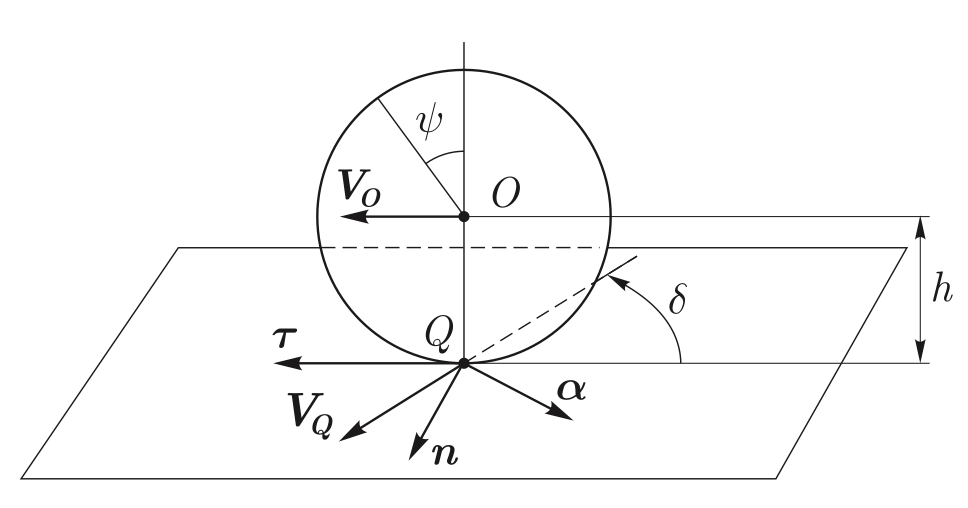
\includegraphics[width=0.75\textwidth]{content/parts/3_friction/diploma/img/art/bor_wheel_scheme.png}
    % 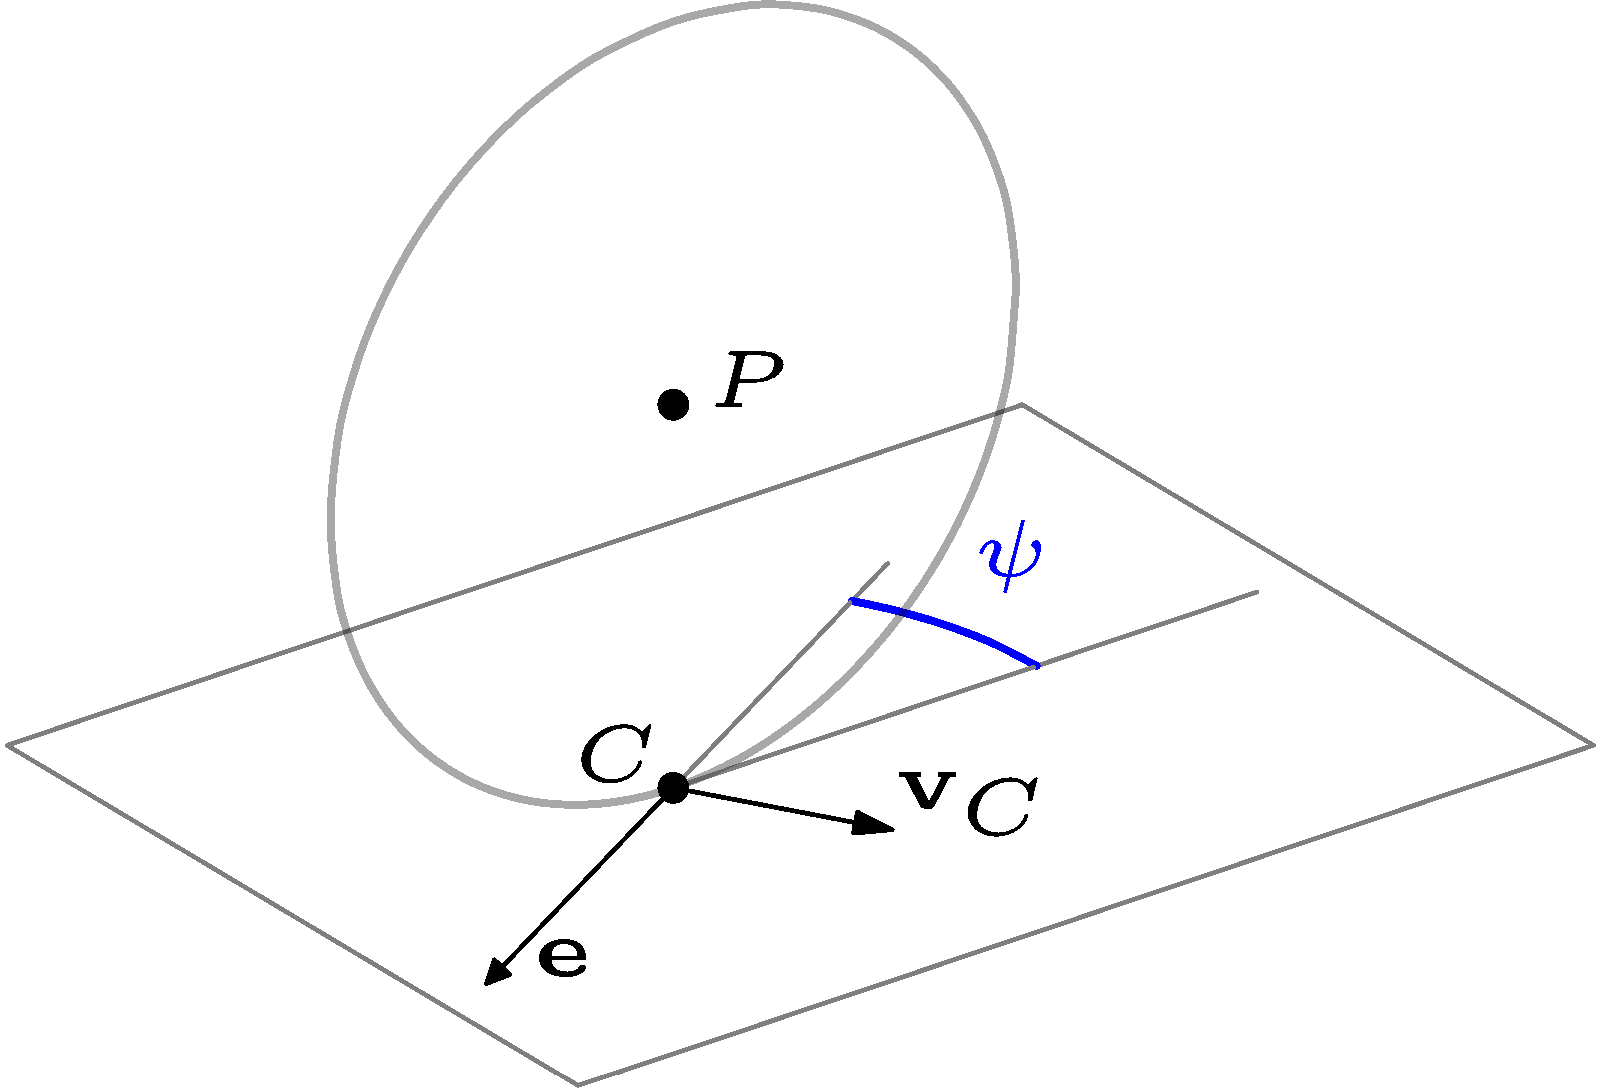
\includegraphics[width=0.5\textwidth]{content/pic/asy/wheel_bor.png}
    \asyinclude[width=0.75\textwidth]{content/pic/asy/wheel_bor.asy}
    \caption{Безынерционная модель колеса}
    \label{fig:bor_wheel_scheme}
\end{figure}

Авторы \cite{Borisov2011} получают уравнения движения для экипажа с произвольным количеством и расположением колес, закрепленных так, что их оси неподвижны относительно платформы, а оси роликов повернуты на произвольные углы относительно плоскостей соответствующих колес (см. фиг.~\ref{fig:bor_vehicle}).

\begin{figure}[ht!]
    \centering
    % 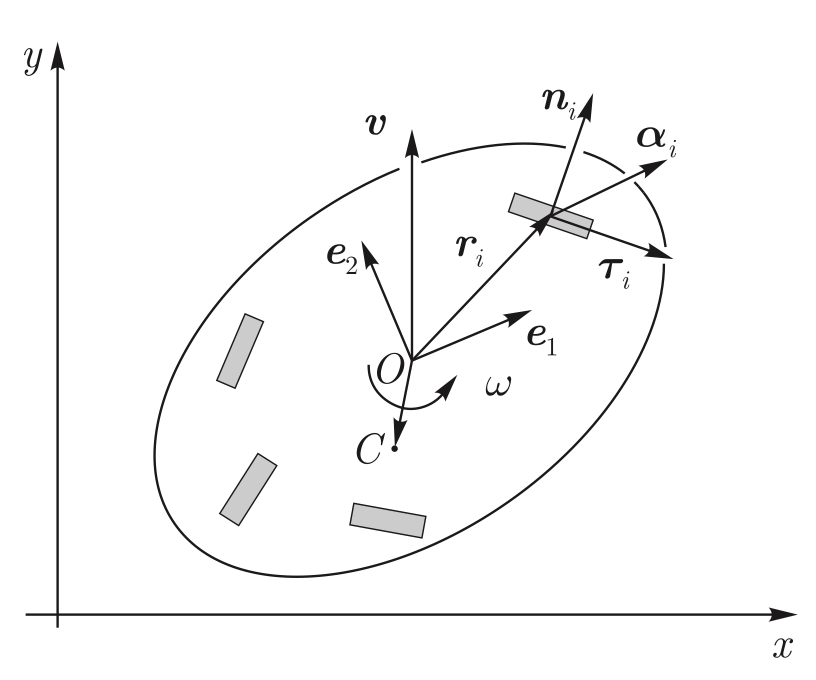
\includegraphics[width=0.75\textwidth]{content/parts/3_friction/diploma/img/art/bor_vehicle.png}
    % 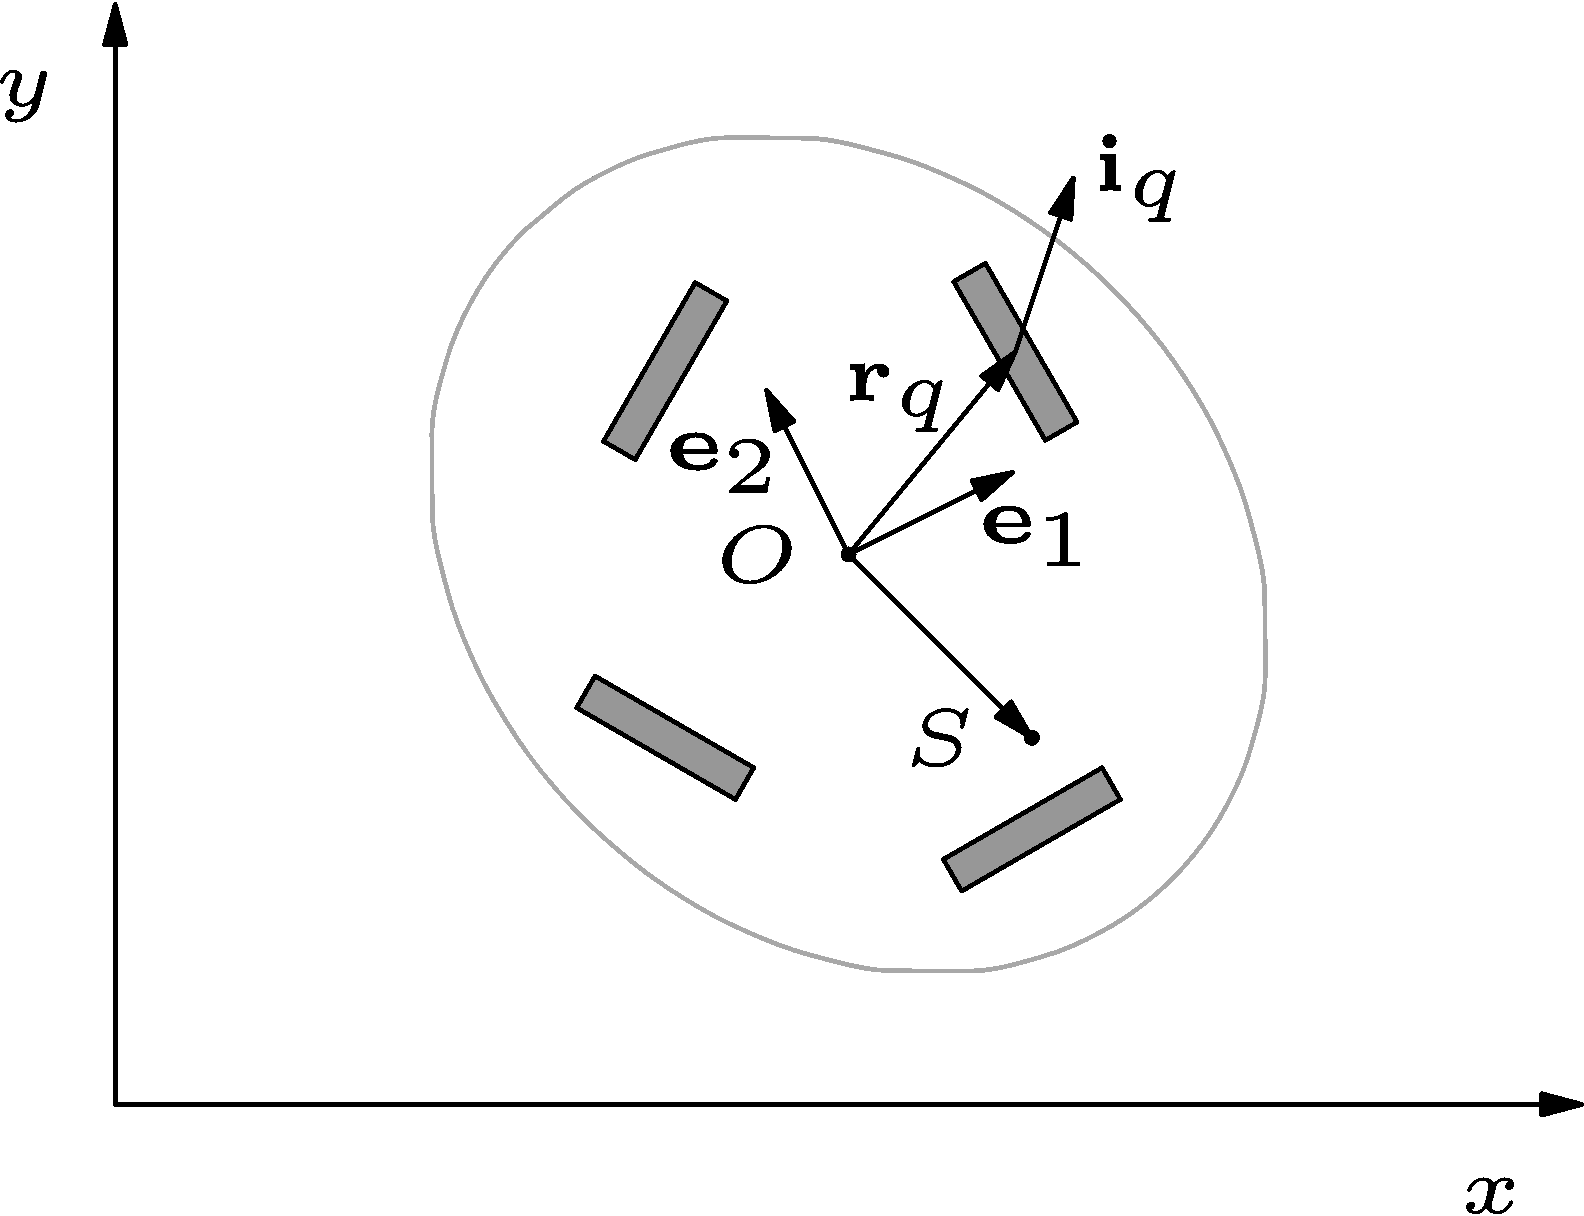
\includegraphics[width=0.75\textwidth]{content/pic/asy/cart_bor.png}
    \asyinclude[width=0.75\textwidth]{content/pic/asy/cart_bor.asy}
    \caption{Безынерционная модель экипажа}
    \label{fig:bor_vehicle}
\end{figure}

Вводится подвижная система отсчета $S\xi\eta$, связанная с платформой экипажа. Центр масс $M$ экипажа может не совпадать с началом $S$ подвижной системы отсчета. В качестве уравнений движения используются уравнения Феррерса. Все векторы в записи уравнений движения двумерны. Уравнения движения по инерции имеют вид:
\begin{eqnarray}\label{eq:bor}
    (\Gamma+mE)\dot{\vec{v}}_S + m\dot{\omega}(J\vec{r}_S+\vec{R})+m\omega J(\vec{v}_S + \omega J\vec{r}_S) = 0,\\
    I_S\dot{\omega} + m(J\vec{r}_S+\vec{R})\cdot\dot{\vec{v}}_S+m\omega\vec{v}_S\cdot\vec{r}_S = 0,\\
    \dot{x} = v_1\cos\theta - v_2\sin\theta, \quad \dot{y} = v_1\sin\theta + v_2\cos\theta, \quad \dot{\theta} = \omega,\\
    \Gamma = \left( \Gamma_{kl} \right), \quad \Gamma_{kl} = \sum_i \frac{I_i}{l_i^2 \cos^2\psi_i}\vec{e}_i^k\vec{e}_i^l, \enspace k,l \in \left\{ 1, 2 \right\} \\
    \vec{R} = m^{-1}\sum_i \frac{I_i}{l_i^2 \cos^2\psi_i}(J\vec{r}_i\cdot \vec{e}_i) \vec{e}_i,
    % \\ I_S = I + \sum_i \frac{I_i}{r_i \cos^2\psi_i}(J\vec{r}_i\cdot \vec{e}_i)^2,
\end{eqnarray}
где: \newline
$x, \ y, \ \theta$ -- координаты точки $S$ и угол поворота платформы экипажа вокруг вертикальной оси,\newline
$\vec{v}_S, \ \omega$ -- вектор скорости точки $S$ и проекция угловой скорости платформы на вертикаль,\newline
$\vec{r}_S$ -- координаты центра масс экипажа в подвижной системе отсчета,\newline
$\vec{r}_i$ -- радиусы-векторы точек закрепления осей колес в подвижной системе отсчета,\newline
$\vec{e}_i^{1,2}$ -- проекции векторов $\vec{e}_i$ а оси $\xi,\eta$ подвижной системы отсчета,\newline
$I_S$ -- суммарный момент инерции системы относительно вертикальной оси, проходящей через начало $O$ подвижной системы отсчета,\newline
% $I$ -- момент инерции платформы относительно той же прямой,\newline
$I_i$ -- моменты инерции колес относительно их диаметров,\newline
$l_i$ -- радиусы колес,\newline
$E$ -- единичная матрица,
$J = \left(\begin{array}{cc}0 & 1\\-1 & 0\end{array}\right)$.

% Данная неголономная модель экипажа также реализована на языке Modelica \cite{ModelicaSpec} как часть упомянутой библиотеки \cite{KosenkoBond}. Таким образом, возможно проведение сравнительного анализа физически-ориентированной и идеализированной моделей и верифкация.

В конфигурации экипажа, рассматриваемой в настоящей работе, центр масс совпадает с началом подвижной системы отсчета $\vec{r}_S = 0$. Кроме того, в силу расположения центров колес в вершинах правильного многоугольника, лежащего в плоскости платформы, а также, поскольку все колеса одинаковы, вектор $\vec{R}$ также равен нулю. В этих условиях второе уравнение системы~\ref{eq:bor} принимает вид $I_S\dot{\omega} = 0$, откуда следует первый интеграл $I_S\omega = \const$. Этот интеграл разрушается при учете инерции роликов, как показано в разделе~$\ref{sect:eqs}$.

Количество степеней свободы безынерционной модели экипажа с $N$ колесами равно $3 + N$, что меньше количества степеней свободы моделей, учитывающих инерцию всех $n$ роликов каждого колеса -- $3 + N(n - 1)$ в постановке без проскальзывания либо $3 + N(n + 1)$ в постановке с голономными связями. В силу более простой структуры, безынерционная модель может быть использована для верификации более сложных моделей экипажа с омни-колесами.